\documentclass[smallextended,envcountsect,envcountsame]{svjour3}
\smartqed
\usepackage[T1]{fontenc}
\usepackage[utf8]{inputenc}
\usepackage{fix-cm,amsmath,amssymb,mathtools,booktabs,array,graphicx,xurl,placeins}
\usepackage{xr-hyper}
\usepackage{hyperref}
\hypersetup{colorlinks=true,linkcolor=blue,citecolor=blue,urlcolor=blue}
\setlength{\emergencystretch}{1em}
\journalname{JOTA}
\renewcommand{\subclassname}{{\bfseries Mathematics Subject Classification (2020)}\enspace}
\newcommand{\E}{\mathbb E}
\newcommand{\Pp}{\mathbb P}
\newcommand{\R}{\mathbb R}
\newcommand{\Cov}{\operatorname{Cov}}
\newcommand{\Risk}{\mathcal R}
\newcommand{\ind}{\mathbf1}
\newcommand{\Law}{\operatorname{Law}}
\newcommand{\asympc}{\asymp}
\raggedbottom

\IfFileExists{ESM_1.aux}{\externaldocument{ESM_1}}{\externaldocument{xref_cache/ESM_1}[ESM_1.pdf]}
\begin{document}
\title{Same Loss and Gradient Covariance, Different Stationary Errors in Adaptive Optimization}
\titlerunning{Pairing and Stationary Error in Adaptive Optimization}
\author{Ihor Kendiukhov}
\authorrunning{Ihor Kendiukhov}
\institute{Ihor Kendiukhov (corresponding author) \at
Institute of Medical Genetics and Applied Genomics, University of T\"ubingen, T\"ubingen, Germany\\
\email{ihor.kendiukhov@student.uni-tuebingen.de}}
\date{}
\hypersetup{pdftitle={Same Loss and Gradient Covariance, Different Stationary Errors in Adaptive Optimization},pdfauthor={Ihor Kendiukhov}}
\maketitle
\begin{abstract}
The average loss and gradient covariance need not determine the long-run
error of an adaptive gradient method. We prove this for AdamW using two
quadratic problems with two interacting parameters and smooth sampling
distributions. Every sampled loss is strongly convex. The two problems
have the same average loss, the same separate distributions of sample
curvature and gradient noise at the average-loss minimum, and the same
gradient covariance at every pair of parameter values. Only the pairing
of curvature and noise differs.

With identical fixed optimizer settings, stationary error decreases in
proportion to the learning rate in one problem but remains bounded away
from zero in the other. Plain stochastic gradient descent has exactly
the same stationary error on both problems. An exact formula explains
how AdamW weights curvature according to the noise magnitude observed
with it. We identify conditions restoring vanishing error, give the
sharp error range in one dimension, extend the construction to a range
of pairings, and quantify a sequential long-memory limit. Simulations of
a discrete example support the mechanism.

The result provides a controlled test of theories of adaptive optimization:
loss and covariance summaries alone can miss a change in the order of
stationary error. The formula identifies additional dependence that such
theories need to retain.
\end{abstract}
\keywords{AdamW \and Stochastic approximation \and Invariant distributions \and Stochastic optimization \and Curvature--noise dependence}
\subclass{62L20 \and 90C15 \and 60J05}

\section{Introduction}
AdamW rescales each gradient coordinate using averages of past gradients
and squared gradients. Its average update can therefore differ from the
average gradient. We ask what information is needed to predict its
stationary error: expected excess loss when the joint distribution of
parameters and moment estimates is unchanged by further updates.

Curvature describes how the gradient changes when the parameters move;
for quadratic losses it is the Hessian matrix. Gradient noise is the
difference between a sampled gradient and its mean. Their separate
distributions do not determine how they occur together. We call this
remaining dependence a \emph{coupling}, or pairing.

We construct two problems that share the average loss, the full separate
Hessian and optimum-noise distributions, and gradient covariance at every
pair of parameter values, including the use of the same sample at both
values. Changing only the pairing makes one averaged update restore the
common optimum and the other repel it in one direction. We prove that
stationary error vanishes in proportion to the learning rate in one
problem but remains bounded away from zero in the other. Plain stochastic
gradient descent has exactly the same stationary error on both.

The two parameters interact: the sampled Hessians do not share an
eigenbasis. The distributions can be smooth, and one fully specified
example has sample condition numbers below ten. Symmetric noise keeps
the optimum a zero of both averaged updates, so the mechanism changes
stability rather than merely shifting that zero. We extend the result
to a range of pairings and identify conditions restoring vanishing error.
The supplementary results quantify error, local return speed and a
sequential long-memory limit. We assert neither a finite-start mixing-time
bound nor a language-model training benefit.

\subsection*{Related Work}
\paragraph{Adaptive Updates and Convergence.}
Adaptive coordinate scaling predates Adam through AdaGrad and ADADELTA
\cite{duchi2011adagrad,zeiler2012adadelta}. Adam uses gradient-moment
averages \cite{kingma2015adam}; AdamW separates weight decay from that
scaling \cite{loshchilov2019adamw}. Sign and variance interpretations
\cite{balles2018dissecting,bernstein2018signsgd} and alternative
denominators such as AdaBelief \cite{zhuang2020adabelief} are established.
Convergence analyses cover nonconvex settings
\cite{zaheer2018adaptive,chen2019adamtype}, averaging-parameter conditions
\cite{zou2019sufficient}, and unchanged Adam updates
\cite{defossez2022simple,zhang2022adam}. Their assumptions do not imply
minimizer consistency for every fixed-memory, constant-step problem.
Our result concerns the specified AdamW denominator, including its shared
history with the gradient.

\paragraph{The Closest Comparisons.}
The averaged Adam field already depends on the whole sampling law
\cite{dj2024}. Its derivative and corrected noise covariance enter a
decreasing-step, averaged-iterate central limit theorem conditional on
convergence to a stable zero \cite{dj2026}. Theorem~4.12 of
\cite{symmetry} concerns fixed isotropic curvature; here sign-symmetric
noise and random curvature preserve the same zero while changing stability.
Stochastic convex failure \cite{reddi}, deterministic AdamW instability
and exact discrete-step conditions
\cite[Proposition~4.3 and Appendix~A.6]{su}, and large-step stability
phenomena \cite{cohen_edge,adaptive_edge,eos} are prior results.
Normalization-dependent floors versus SGD under multiplicative noise also
precede us \cite{singh}; that comparison changes the normalization rule.
Our distinction is the same AdamW update, with fixed positive offset and
decay, having vanishing versus persistent stationary error when only the
pairing changes. The average loss, full gradient covariance kernel and both
complete Hessian and noise marginals remain fixed. The moment averages
continue fluctuating at the minimum even as the step vanishes.

\paragraph{Classical Methods and Stationary Error.}
Stochastic approximation \cite{robbinsmonro1951}, its differential-equation
and stability methods \cite{kushneryin2003,benaim1999,borkarmeyn2000},
unstable-point avoidance \cite{pemantle1990}, and constant-step stationary
limits \cite{fortpages,ddb,chenmoumaguluri2022} supply established tools.
We prove their required gradient-history estimates rather than claiming new
Gaussian-limit or covariance methods. The additional work controls every
stationary distribution satisfying the algorithm's moment constraints,
including a case where
the optimum repels the averaged dynamics. Exact SGD balance identities
\cite{yaida2019} presuppose stationarity; martingale corrections handle
dependent noise \cite{fort2015}. Iterate averaging changes fluctuations
\cite{polyakjuditsky1992,mouetal2020}; our error concerns an unaveraged
stationary iterate. Classical rearrangement inequalities
\cite{cambanissimonsstout1976} give our scalar extrema after deriving the
optimizer-specific response weight, not a new general coupling inequality.

\paragraph{Diffusion Models and Memory.}
Finite-time stochastic differential equation approximations
\cite{litaie2017} extend to adaptive methods and scaling rules
\cite{malladi,compagnoni}. Their Adam limits let memory parameters approach
one as the step decreases; our main theorem fixes memory and the sampling
law. These approximations already describe interactions between adaptive
normalization and noise; different memory scalings can retain different
parts of that interaction. Finite-time approximation alone does not justify
exchanging long-time and small-step limits. Our separate long-memory result takes the small-step
limit first, without covering every simultaneous scaling. The example
challenges descriptions retaining only the matched summaries, not diffusion
models that retain additional dependence information.

\paragraph{Noise, Curvature and Adaptive Bias.}
SGD diffusion models connect fluctuations to approximate Bayesian inference
and noise scale \cite{mandt2017,smithle2018}, and anisotropic noise to
probability currents \cite{chaudharisoatto2018}. Curvature--noise tradeoffs
\cite{thomas}, Adam covariance with a population replacement for the
random denominator \cite{liu2021}, bias near minimizer manifolds under
another memory scaling \cite{liwenlyu}, preconditioning limits \cite{das},
and discrete-update regularization \cite{cattaneo} are established.
Keeping the realized denominator random distinguishes our exact response
formula; the matched-law stationary error orders distinguish the
construction.

\paragraph{Connections to Transformers and Limits.}
Heavy-tailed gradient noise \cite{simsekli,zhang_attention} and Hessian
block differences \cite{zhang_hessian} offer other explanations for
adaptive optimization. SGD--Adam gaps can persist without sampling noise
\cite{kunstner2023noise}, and optimization gains need not improve
generalization \cite{wilson2017marginal}. Our bounded-noise examples fix
the entire Hessian law and isolate an additional dependence. They establish
neither a full explanation of transformer optimization nor a language-model
or generalization benefit. Bounded noise makes heavy tails unnecessary for
this particular separation, without disputing their empirical role in
neural-network training.



Appendices A--E contain the essential proofs in this paper. Appendices
F--I and Section S1, including the extension statements and proofs and supporting numerical records, are
in Online Resource~1. Online Resource~2 provides the scientific code and
recorded data used for the numerical results.

\section{The Algorithm and the Quantities Held Fixed}
At each update draw $(A_n,e_n)$ independently from the same joint
distribution. The matrix gives sample curvature, and the vector gives
the sample gradient at zero. In our examples zero minimizes the average
loss. These samples define
\[
 \begin{gathered}
 \ell(u;A,e)=\tfrac12u^\top Au+e^\top u,\qquad g(u;A,e)=Au+e,\\
 0<h_{\min}I\preceq A\preceq h_{\max}I,
 \end{gathered}
\]
with bounded symmetric $A$ and bounded $e$. Fix
$0\leq\alpha<\rho=\sqrt\beta<1$ and $\epsilon,\lambda>0$.
We use the following coordinatewise AdamW update at a constant learning rate:
\begin{align}
 m_{n+1}&=\alpha m_n+(1-\alpha)g(u_n;A_{n+1},e_{n+1}),\nonumber\\
 v_{n+1}&=\beta v_n+(1-\beta)g(u_n;A_{n+1},e_{n+1})^{\odot2},
 \label{eq:native}\\
 u_{n+1}&=(1-\eta\lambda)u_n
                -\eta\frac{m_{n+1}}{\sqrt{v_{n+1}}+\epsilon}.
 \nonumber
\end{align}
Here $m$ and $v$ are exponential averages of gradients and squared gradients,
$\epsilon$ is the positive denominator offset, and $\lambda$ is weight
decay. The initial bias correction is omitted. Put
\[
 w_j=(1-\alpha)\alpha^j,\quad d_j=(1-\beta)\beta^j,\quad
 C_*^2=\sum_{j\geq0}\frac{w_j^2}{d_j}
 =\frac{(1-\alpha)^2}{(1-\beta)(1-\alpha^2/\beta)}.
\]
The moment constraints $v_i\geq0$, $m_i^2\leq C_*^2v_i$ define the set
we call the \emph{native cone}. Zero initial moment estimates satisfy these
constraints, and every update preserves them. For $\eta\lambda\leq1$,
every stationary distribution in this set is supported on
$\|u\|_\infty\leq C_*/\lambda$. Such stationary distributions exist.
Appendix~\ref{app:transfer} proves these bounds and relates the update with
its actual past gradients to its averaged description.

A \emph{law} means a probability distribution. We use \emph{invariant}
and \emph{stationary} interchangeably: an update leaves the joint
distribution of parameters and moment estimates $(u,m,v)$ unchanged.
``Every invariant selection'' means any choice of stationary
distribution at each allowed learning rate. We assume neither uniqueness
nor a rate at which a run approaches stationarity. The risk in the formal
statements is stationary error, measured as expected excess average loss.

We hold the full separate distributions of $A$ and $e$ fixed. In our examples
$\E e=0$ and every cross moment $\E[A_{ij}e_k]=0$. With $\bar H=\E A$,
\begin{equation}\label{eq:matched-kernel}
 \begin{gathered}
 L(u)=\tfrac12u^\top\bar H u,\qquad \E g(u)=\bar H u,\\
 \Cov(g(u),g(v))=\E[(A-\bar H)uv^\top(A-\bar H)]+\E ee^\top.
 \end{gathered}
\end{equation}
The covariance uses the same sampled loss at $u,v$. For quadratics, the
displayed moments and separate distributions therefore fix it at every pair
of parameter values. The joint distribution of curvature and noise, and
their higher cross moments, can still differ.

\begin{theorem}[A fixed smooth matched pair with different stationary risk orders]
\label{thm:main}
For every admitted fixed $\alpha,\beta,\epsilon,\lambda$, there are two
fixed smooth compactly supported joint laws on
$\operatorname{Sym}_2\times\R^2$, called independent and coupled, such that:
\begin{enumerate}
 \item All sample Hessians are uniformly positive definite; their law is
 full dimensional and independent sample Hessians fail to commute almost
 surely. The two laws share the complete separate Hessian and optimum-noise
 marginals and every quantity in \eqref{eq:matched-kernel}.
 \item Both joint laws are invariant under each individual coordinate
 sign flip of $e$ with $A$ unchanged, and under simultaneous coordinate
 exchange $(A,e)\mapsto(PAP,Pe)$. The common optimum $0$ is a zero of
 both averaged AdamW fields.
 \item For every invariant native-cone selection,
 \[
\begin{gathered}
  \Risk_{\rm independent}(\eta)=C\eta+o(\eta),\quad 0<C<\infty,
\\
   0<\underline R\leq\Risk_{\rm coupled}(\eta)\leq\overline R<\infty
\end{gathered}
 \]
 for all sufficiently small $\eta$. Here $\Risk=\E L(u)$.
 \item Plain SGD with the same decay has exactly equal stationary
 covariance matrices and quadratic risks for the two laws throughout a
 common stable step interval; both risks have order $\eta$.
\end{enumerate}
All sample laws, supports, conditioning constants and optimizer parameters
are fixed before the step limit. The risk ratio is of order $1/\eta$.
\end{theorem}

The proof constructs the pair explicitly. Sections~\ref{sec:field}--\ref{sec:phases}
give the matrices and explain why one case is stable and the other is not.
The appendices prove the stationary results for the actual AdamW update.
Conditioning and
cross-sample curvature spread are finite for each example; they are not
uniformly bounded over every memory choice or requested spectral margin.

\section{How Gradient Noise Reweights Curvature}\label{sec:field}
The key quantity is how the average AdamW update changes near the minimum.
To compute it, fix the parameter $u$ while averaging past gradient samples.
For a complete sample history $Z$, define
\[
\begin{gathered}
 f_i(u,Z)=\frac{\sum_{j\geq0}w_j((A_{-j}u)_i+e_{i,-j})}
 {\sqrt{\sum_{j\geq0}d_j((A_{-j}u)_i+e_{i,-j})^2}+\epsilon},
 \\ F(u)=\E f(u,Z),\quad G(u)=\lambda u+F(u).
\end{gathered}
\]
Noise marginals are symmetric and nonzero with positive probability.
Let $R_{\max}=\max_i\operatorname{ess\,sup}|e_i|$,
$R_i=|e_i|$, $V_{i,-j}=\sum_{k\ne j}d_kR_{i,-k}^2$, and, for
$0\leq r\leq R_{\max}$, put
\begin{equation}\label{eq:psi}
 \Psi_i(r)=\sum_{j\geq0}w_j\E\left[
 \frac{V_{i,-j}}{x(x+\epsilon)^2}
       +\frac{\epsilon}{(x+\epsilon)^2}\right],
 \qquad x=\sqrt{V_{i,-j}+d_jr^2}.
\end{equation}
The expectation over other times depends only on the distribution of $R_i$.
The function $\Psi_i$ will give the weight applied to curvature in coordinate
$i$. The term \emph{susceptibility kernel} below refers to this curvature
weight in the local slope of the averaged update.

\begin{proposition}[Exact curvature-weighting formula]\label{prop:rowkernel}
Every $\Psi_i$ is positive, continuous and strictly decreasing, with
$\epsilon/(R_{\max}+\epsilon)^2\leq\Psi_i\leq1/\epsilon$.
The exact origin field derivative is
\begin{equation}\label{eq:rowkernel}
 J_{ik}=\partial_kF_i(0)=\E[A_{ik}\Psi_i(|e_i|)].
\end{equation}
Only marginal noise symmetry is needed for this identity; sample Hessians
need not commute. Positive definite $A$ alone need not make $J$ positive stable.
\end{proposition}

The proof differentiates the quotient built from past gradients. Cross
terms involving different times average to zero: they contain a symmetric
noise sign but not the curvature sampled at that same time. The remaining
terms give \eqref{eq:psi}; both decrease with $r$.
Appendix~\ref{app:kernel} gives the details. The formula says that curvature
observed with smaller noise receives greater weight. Replacing the random
denominator by its population approximation would lose this dependence.

\begin{theorem}[Exact error range in one dimension]\label{thm:scalar}
In dimension one fix complete bounded marginals $H\in[h_{\min},h_{\max}]$
and symmetric nonzero $e$. Allow every signed coupling with $\E He=0$.
Let $\mu=\E H$, $\chi=\E[H\Psi(|e|)]$, and let $D_\epsilon>0$ be the
origin Green--Kubo variance of the native action. Every invariant selection has
\[
 u/\sqrt\eta\Rightarrow N\!\left(0,\frac{D_\epsilon}{2(\lambda+\chi)}\right),
 \qquad C(H,e):=\lim\frac{\E L(u)}\eta
       =\frac{\mu D_\epsilon}{4(\lambda+\chi)}.
\]
All positive absolute scaled moments converge. If $a,b$ are the generalized
quantiles of $H,|e|$, define
\[
 \chi_{\min}=\int_0^1a(t)\Psi(b(t))dt,
 \qquad \chi_{\max}=\int_0^1a(t)\Psi(b(1-t))dt.
\]
The complete attainable risk interval is
\[
 \frac{\mu D_\epsilon}{4(\lambda+\chi_{\max})}
 \leq C(H,e)\leq
 \frac{\mu D_\epsilon}{4(\lambda+\chi_{\min})}.
\]
Opposite curvature/magnitude ranks minimize risk; equal ranks maximize it.
Both extrema and all intermediate values are attainable, and their ratio is
at most $h_{\max}/h_{\min}$. The endpoints differ strictly when both
marginals are nondegenerate.
\end{theorem}

The theorem gives the full range of possible leading errors in one
dimension. Pairing large curvature with small noise gives the lowest error;
pairing large curvature with large noise gives the highest. The step that
bounds an average product from its separate distributions is classical
\cite{cambanissimonsstout1976}. The AdamW-specific part is \eqref{eq:rowkernel} and
its decreasing weight. Appendices~\ref{app:kernel}--\ref{app:transfer}
prove that the averaged update points inward and that the actual stationary
error has the stated limit. Section~\ref{sec:phases} proves exact equality
of SGD errors for the matrix examples as well.

\section{Constructing Vanishing and Persistent Error}\label{sec:phases}
Let the vector noise have magnitudes $(0,a)$ or $(a,0)$ with equal
probabilities, with fair independent coordinate signs. Its coordinate
marginals are identical. For the common kernel let
\[
 K=\frac{\Psi(0)}{\Psi(a)}>1.
\]
Choose any fixed $M,b$ with
\begin{equation}\label{eq:construction-window}
 1<\sqrt M<K,\qquad
 \frac{K+M}{K+1}<b<\sqrt M,
 \qquad \Delta=b(K+1)-(K+M)>0.
\end{equation}
The interval is nonempty because $(\sqrt M-1)(\sqrt M-K)<0$.
Set
\[
 H_1=\begin{pmatrix}1&b\\b&M\end{pmatrix},\quad
 H_2=\begin{pmatrix}M&b\\b&1\end{pmatrix},\quad
 s>\frac{2\lambda}{\Psi(a)\Delta}.
\]
Both matrices are positive definite and do not commute; their commutator has nonzero entry
$2b(1-M)$. In the coupled law use $A=sH_1$ for magnitude $(0,a)$ and
$A=sH_2$ for $(a,0)$. In the independent law draw the same equally
weighted Hessian distribution independently of the entire noise vector.
Fair signs make every $\E[A_{ij}e_k]$ vanish. This proves all matching
claims in \eqref{eq:matched-kernel}.

\begin{figure}[htbp]
\centering
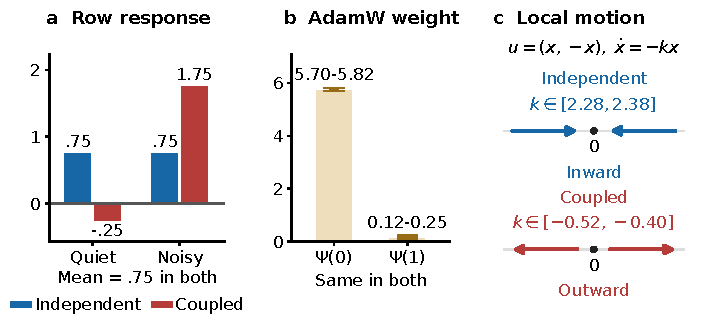
\includegraphics[width=\linewidth]{figures/pairing_mechanism.pdf}
\caption{How a different pairing reverses mean motion in the concrete
example of Section~\ref{sec:matrix-experiment}. Both problems have the same
separate curvature and noise distributions and the same gradient covariance.
\textbf{a:} For displacement $u=(x,-x)$, bars give the mean coordinate
gradient per unit coordinate displacement, conditioned on that coordinate
having zero noise (quiet) or unit noise (noisy). Equivalently, they show
$\E[(Au)_i/u_i\mid |e_i|]$. A negative bar gives an outward descent component;
it is not a negative Hessian eigenvalue. Ordinary averaging gives $.75$ in
both cases. \textbf{b:} AdamW's local curvature weights are the same in both
problems, but the quiet coordinate receives much more weight. These weights
average over the full noise history; they are not instantaneous inverse-noise
factors. Caps show deterministic certified bounds, not confidence intervals.
\textbf{c:} After including weight decay, the local mean motion is
$\dot x=-kx$. The weighted quiet contribution now makes the coupled case
repel along this direction. Arrows show direction only in this local
linearization, not simulated trajectories. Plotting code was developed with OpenAI Codex; displayed quantities are derived from certified calculations.}
\label{fig:copulas}
\end{figure}

The coupled Jacobian is
\[
 J_c=\frac{s\Psi(a)}2
 \begin{pmatrix}K+M&b(K+1)\\b(K+1)&K+M\end{pmatrix}.
\]
Thus $\lambda I+J_c$ has negative eigenvalue
$\lambda-s\Psi(a)\Delta/2$ on $v=(1,-1)/\sqrt2$, and a positive
eigenvalue on the symmetric direction. The origin is a saddle for
$\dot u=-G(u)$: motion is pushed away in one direction and pulled back in
the other. In the independent case the Jacobian is
\[
 J_r=c\bar H,\qquad c=\tfrac12(\Psi(0)+\Psi(a))>0,
 \qquad \bar H=\E A,
\]
which is positive definite after adding decay. These local calculations
alone do not prove the stationary errors. We must also show that the
independent update pulls inward globally, and that random updates cannot
remain concentrated at the repelling minimum in the coupled case.

\paragraph{Why the independent case has small error.}
In the independent law, $A-\bar H$ has the same distribution as its negative.
At fixed $u$, each gradient coordinate has a symmetric distribution about
$m_i=(\bar H u)_i$. Odd-monotone scalar normalization implies
$m_iF_i(u)\geq0$. Consequently
\begin{equation}\label{eq:restoring-lyapunov}
 u^\top\bar H G(u)\geq\lambda u^\top\bar H u.
\end{equation}
This inequality shows that the average loss decreases along the averaged
dynamics away from the minimum. It is a Lyapunov bound, meaning a bound
that controls distance from the minimum. It first gives stationary moment
bounds for the actual update; a diffusion limit then gives the precise
leading error. With common origin variance $D>0$,
the independent limiting covariance and risk coefficient are
\begin{equation}\label{eq:reference-limit}
 S_r=\tfrac D2(\lambda I+c\bar H)^{-1},\qquad
 C_r=\tfrac D4\operatorname{tr}[\bar H(\lambda I+c\bar H)^{-1}].
\end{equation}
Appendix~\ref{app:reference} proves \eqref{eq:restoring-lyapunov} and
derives the result for the update using its actual past gradients.

\paragraph{Why the coupled case retains positive error.}
Swapping the two coordinates leaves the problem unchanged. This symmetry
makes the antisymmetric drift component divisible by
$y=v^\top u$: $|G_v(u)|\leq L|y|$ on the enlarged native box. Its
negative local derivative gives $yG_v(u)\leq-a_0y^2$ near zero. At the
origin a bounded adjustment for past noise, called the Poisson corrector,
is linear in the realized noise signs, with
a uniformly positive coefficient for the fresh sign. Hence the variance of
the remaining centered random update in direction $v$ has a positive lower
bound for every old history. For the test function $\log(y^2+h\eta)$,
repulsion and this fresh noise give a positive expected change near zero,
with a bounded negative change elsewhere. Stationarity requires the average
change to be zero, forcing positive probability outside a fixed neighborhood
of the minimum. Appendix~\ref{app:repulsion} proves this for the actual
chain, without assuming an unproved rate of approach to stationarity or
independence from past gradients.

\paragraph{Smooth distributions and the SGD comparison.}
Add the same independent small fixed smooth symmetric matrix jitter to $A$
and iid symmetric smooth coordinate jitters to $e$ in both laws. Choose a
matrix perturbation from a smooth density that depends only on its norm.
This preserves symmetry under reflection and coordinate exchange. The joint
densities are smooth in every matrix and noise direction, while all matching
conditions and sign symmetries remain. Small enough fixed perturbations
preserve positive sample curvature and the strict stability signs. The
independent law retains matrix central symmetry and independence from $e$.

For SGD put $T=I-\eta(A+\lambda I)$. In a common contractive step interval
the invariant covariance uniquely solves
\begin{equation}\label{eq:SGD-matrix}
 \Sigma=\E[T\Sigma T^\top]+\eta^2\E ee^\top.
\end{equation}
All cross terms vanish; this equation depends only on the fixed separate
distributions. Both stationary covariances and errors agree exactly and are of order
$\eta$. Appendix~\ref{app:reference} completes smoothing and this matrix
argument, proving Theorem~\ref{thm:main}.

\subsection{Changing the Pairing Continuously}
\label{sec:continuous-copula}
The distinction is not restricted to two isolated pairings. Mixing their
sampling distributions gives a continuous range of dependence choices,
all with exactly the same listed summaries. Fix one smooth pair of
Theorem~\ref{thm:main}, with joint sample laws $\mathcal P_0,\mathcal P_1$, and put
$\mathcal P_\theta=(1-\theta)\mathcal P_0+\theta\mathcal P_1$,
$0\leq\theta\leq1$. Each time sample is drawn independently from this
mixture. Let $k_{0,-}>0$ and $k_{1,-}<0$ be the endpoint antisymmetric
eigenvalues of $\lambda I+DF(0)$; their symmetric eigenvalues are positive.

\begin{corollary}[Ranges of pairings with different stationary errors]
\label{cor:continuous-copula-phases}
Every $\mathcal P_\theta$ has the same complete Hessian/noise marginals,
population loss and gradient covariance kernel. Its local origin threshold
is exactly
\begin{equation}\label{eq:copula-local-threshold}
 \theta_* =\frac{k_{0,-}}{k_{0,-}-k_{1,-}}\in(0,1).
\end{equation}
The origin is locally exponentially stable for $\theta<\theta_*$ and a
hyperbolic saddle for $\theta>\theta_*$. There is a fixed $\theta_0>0$
such that every $\theta\in[0,\theta_0]$ has stationary risk
$C_\theta\eta+o(\eta)$ with $C_\theta>0$, for every invariant selection.
Every fixed $\theta>\theta_*$ has stationary risk $\Theta(1)$ for every
selection. Plain SGD has exactly the same stationary covariance and
order-$\eta$ risk for the whole family at sufficiently small common steps.
No stationary classification is asserted at $\theta_*$ or throughout the
remaining locally stable interval $(\theta_0,\theta_*)$.
\end{corollary}
The complete proof is in Appendix~\ref{app:continuous}. Near the independent
endpoint we prove vanishing stationary error; beyond the local stability
threshold we prove a positive floor. The interval between these ranges and
the threshold itself are not fully classified. A local stability change
does not determine a finite-learning-rate transition or the dynamics
exactly at the threshold.

Online Resource~1, Section~\ref{sec:supplementary-extensions}, gives the
matched-return-speed comparison, a sequential long-memory expansion, and
the extension of the exact scalar error range to an interacting matrix
family. Their full statements, assumptions and proofs are retained there.

\section{Numerical Tests}
For each prospective experiment, the code, settings and prediction intervals
were fixed before its simulations. The analysis includes every declared
setting and every recorded run. We estimate uncertainty by resampling whole
independent simulation runs, keeping all paired conditions together.
The resulting bootstrap intervals are approximate. They do not prove that
the runs have reached stationarity or bound how fast this happens.
The reproducibility archive contains the raw observations and run records.

\subsection{The Two-Dimensional AdamW Experiment}\label{sec:matrix-experiment}
The experiment samples the two matrices
\[
 H_1=\begin{pmatrix}1&1.25\\1.25&3\end{pmatrix},\qquad
 H_2=\begin{pmatrix}3&1.25\\1.25&1\end{pmatrix},\qquad a=1,
\]
with $\alpha=.1$, $\beta=.2$, $\epsilon=.03$, $\lambda=.1$ and no
Hessian scaling. The displayed optimizer decimals label their exact
double-precision computer representations. Appendix~\ref{app:certificate}
specifies these rational values and the calculation used to bound the
curvature weights. Before simulating any two-dimensional trajectory, a
deterministic calculation over finite histories, with bounds for omitted
history and rounding, gave
\[
 \Psi(0)\in[5.703200,5.816980],\qquad
 \Psi(1)\in[.126867,.240647].
\]
Propagating the underlying unrounded intervals with outward rounding gives bounds on the
eigenvalues of $\lambda I+J$, whose signs determine local stability
(Table~\ref{tab:field-stability}):
\begin{table}[htbp]
\caption{Certified Bounds for the Local Drift Eigenvalues}\label{tab:field-stability}
\centering

\begin{tabular}{ccc}
\toprule
Law & Antisymmetric direction & Symmetric direction\\
\midrule
Coupled & $[-.516114,-.402334]$ & $[6.785694,7.155475]$\\
Independent & $[2.286275,2.371610]$ & $[9.573861,9.943642]$\\
\bottomrule
\end{tabular}
\end{table}
The sample Hessian eigenvalues are approximately $.399219,3.600781$, with
condition number $9.019565<10$; the population eigenvalues are $.75,3.25$.
The mechanism is visible on $u=(x,-x)$. In the coupled law the quiet
coordinate has deterministic sample-gradient component $-.25u_i$, pointing
outward in that coordinate, while the noisy coordinate has $1.75u_i$.
The population component remains $.75u_i$ inward. AdamW gives greater
weight to the quieter coordinate. This reverses the restoring force in
the antisymmetric direction:
\[
 \lambda+\tfrac12[-.25\Psi(0)+1.75\Psi(1)]<0.
\]
An explicit smooth instance at these optimizer settings uses independent
smooth matrix and independent symmetric coordinate perturbations at fixed scale
$\tau=2^{-20}$. Appendix~\ref{app:reference} specifies their densities and
proves $\|J_\tau-J_0\|_{\rm op}<.1$, preserving every stability sign and
sample condition number below ten. Thus the smoothing size is specified
explicitly. The simulations here use the original discrete law; the result
for smooth sampling distributions is proved separately.

The study fixes learning rates $10^{-3},2\cdot10^{-4},4\cdot10^{-5}$,
256 paired simulation runs, and starts $0,\pm(.05,-.05)$ with zero
moment estimates. For AdamW and SGD under both pairings, we record 17
observations in each time window $16{:}32$, $48{:}64$, $112{:}128$, using
time $t=n\eta$. The 432 primary quantities specified before simulation
include all errors, paired differences, exact SGD comparisons, differences
between starts and time windows, and normalized differences between adjacent
learning rates. Their approximate simultaneous confidence intervals account
for the whole set. Descriptive ratios and coordinate means have no such
simultaneous-coverage claim.

All 12 settings and all 612 snapshots completed without a recorded arithmetic
failure. The following display uses the previously specified zero start
and final observation window (Table~\ref{tab:matrix-errors}):
\begin{table}[htbp]
\caption{Stationary-Error Displays at the Prespecified Final Window}\label{tab:matrix-errors}
\centering

\small
\begin{tabular}{cccc}
\toprule
$\eta$ & \shortstack{Independent\\AdamW error} & \shortstack{Coupled\\AdamW error} & \shortstack{Coupled/\\independent ratio}\\
\midrule
$10^{-3}$ & $1.169172\cdot10^{-4}$ & $.2079983$ & $1779\ [1723,1838]$\\
$2\cdot10^{-4}$ & $2.082282\cdot10^{-5}$ & $.2114666$ & $10156\ [9850,10491]$\\
$4\cdot10^{-5}$ & $3.975007\cdot10^{-6}$ & $.2120988$ & $53358\ [51701,55075]$\\
\bottomrule
\end{tabular}
\end{table}
Each ratio has an approximate 95\% interval with endpoints rounded outward;
these intervals are not simultaneous across ratios.
All 27 paired coupled-minus-independent AdamW error differences have positive
lower endpoints in the approximate simultaneous band for all 432 quantities.
All 27 SGD pairing differences and all 54 comparisons with the exact nominal
SGD stationary predictions have intervals containing zero in that band.
The zero-start final-window SGD errors
under the two pairings are respectively
$(2.355295,2.357937)\cdot10^{-4}$,
$(4.677611,4.678263)\cdot10^{-5}$, and
$(9.293840,9.293543)\cdot10^{-6}$.
These exact nominal controls use decimal-rational coefficients; they check
statistical compatibility and are not identities for native floating-point
stationary laws.

The checks also show effects of the finite observation time and learning
rate. Four of 72 differences between starts and two of 72 differences
between time windows exclude zero in the primary simultaneous band. These
involve early coupled AdamW at the two smaller learning rates. Similar late
errors from different starts do not prove that the chain moves between its
two symmetric states. Of 72 normalized adjacent-rate differences, 22 exclude
zero: 16 coupled raw-error differences and six independent AdamW
error/$\eta$ differences. Coupled late error increases by about 2\% across
the grid, and the independent error coefficient also changes. The large
separation at a common observation clock supports the mechanism. Three
learning rates do not prove the limiting scaling, bound the finite-step
error, or determine the numerical value of the stationary error floor.

\begin{figure}[htbp]
\centering
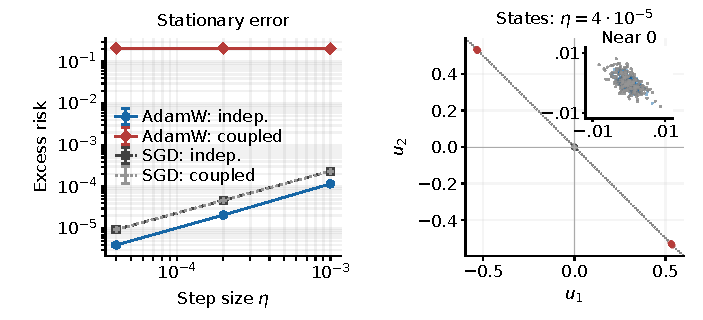
\includegraphics[width=\linewidth]{figures/matrix_phases.pdf}
\caption{Two-Dimensional problems with the same listed summaries but
different curvature/noise pairings, using the discrete sampling law.
Left: all four zero-start final-window error displays, with approximate
simultaneous 95\% error bars for the 432 primary quantities (often smaller than the symbols).
Lines connect observed means; no exponent is fitted. Right: every terminal
state at the finest step, retaining all 256 zero-start replicas for
each method/pairing. The inset shows the clouds near the minimum. These
plots do not prove switching between states or convergence to stationarity.
The error separation for smooth sampling distributions is proved separately. Plotting code was developed with OpenAI Codex; displayed quantities are derived from recorded numerical outputs.}
\label{fig:matrix-phases}
\end{figure}

The supporting scalar study, exploratory time-correlation checks,
and earlier crossover disagreements are retained in Online Resource~1,
Appendix~\ref{app:supporting-studies}. They are not needed for the main
matched-pair theorem.

\section{Conclusions}
For these quadratic problems, the shared loss and covariance summaries
determine SGD's stationary error but do not even determine whether AdamW's
stationary error tends to zero with the learning rate. The curvature-weight
formula identifies the missing dependence. Independence of curvature and
noise, together with the stated matrix symmetry, is one condition that
restores vanishing error.

The result is useful as a controlled test of what a theory of learning
dynamics needs to describe. It isolates one dependence that average loss
and covariance cannot capture, shows how to calculate its effect, and
provides examples against which simplified predictions can be checked.
Whether the same mechanism matters in a trained language model requires
separate evidence.

The main pair is two dimensional and deliberately constructed. The universal
construction may need large conditioning or curvature spread; the explicit
short-memory instance has sample condition numbers below ten. Memory remains
fixed, and all stationary statements refer to the moment constraints
specified in Section~2. Smoothing removes discrete atoms but does not make
the constructed example representative of a trained transformer. We have
not bounded the time to escape the origin or reach stationarity, proved a
unique stationary distribution in the coupled case, or demonstrated a
neural-training intervention. The long-memory result also prevents a direct
extrapolation of the measured short-memory effect to language-model settings.

The appendices give complete proofs, including the adjustment for past
gradients, the positive-error argument and the explicit smooth example.

\appendix
\section{The Exact Response Kernel and Best Possible Scalar Bounds}\label{app:kernel}

The response kernel measures how strongly the averaged update reacts to a
small parameter change. Fix one coordinate, omit its index, and let $R_j=|e_{-j}|$,
$V=\sum_jd_jR_j^2$, $D_V=\sqrt V$. Since independent time samples have
$\Pp(R>0)>0$, both $V$ and each $V_{-j}=V-d_jR_j^2$ are positive
almost surely. Differentiate the frozen quotient in direction $k$:
\[
 \partial_kf_i(0,Z)=
 \frac{\sum_jw_jA_{ik,-j}}{D_V+\epsilon}
 -\frac{(\sum_lw_le_{i,-l})(\sum_jd_je_{i,-j}A_{ik,-j})}
 {D_V(D_V+\epsilon)^2}.
\]
For $l\ne j$, condition on all other times and $|e_{i,-l}|$. The
corresponding product contains $e_{i,-l}$ but not the curvature from that
same sample. Its conditional expectation is zero because the noise
marginal is symmetric. No sign symmetry conditional on that absent
curvature is needed. The surviving same-sample terms are
\[
 \sum_j w_j A_{ik,-j}
 \frac{V-d_jR_j^2+\epsilon\sqrt V}{\sqrt V(\sqrt V+\epsilon)^2}.
\]
Condition each on its own $(A_{ik,-j},R_j)$ and average other times.
This gives \eqref{eq:rowkernel} and \eqref{eq:psi}.

To justify differentiating inside the expectation, use the weighted
square-sum norm on gradient histories $\|x\|_d^2=\sum_jd_jx_j^2$. The numerator
$n(x)=\sum_jw_jx_j$ has representing vector of norm $C_*$. The map
$T(x)=n(x)/(\|x\|_d+\epsilon)$ is continuously differentiable ($C^1$), including derivative
$n/\epsilon$ at zero, with a bounded Lipschitz derivative: its change is at
most a constant times the change in the history. Bounded affine gradient histories
therefore allow differentiation under expectation.
The own-time factor is at most $1/(D_V+\epsilon)\leq1/\epsilon$;
its sum is uniformly bounded by the summable weights.

For $v>0$, both
\[
 \frac{v}{x(x+\epsilon)^2},\qquad
 \frac{\epsilon}{(x+\epsilon)^2},\qquad x=\sqrt{v+d_jr^2},
\]
are strictly decreasing with $r\geq0$. The $j=0$ term has positive
weight, including when $\alpha=0$. Dominated convergence proves continuity;
strictness of this one term proves strict monotonicity of $\Psi$.
Because $D_V\leq R_{\max}$ after each substituted $r\leq R_{\max}$,
\[
 0<\frac{\epsilon}{(R_{\max}+\epsilon)^2}
       \leq\Psi(r)\leq\frac1\epsilon.
\]

\paragraph{Why scalar drift points toward zero.}
For a numerator summand at age $j$, condition on all other times and put
$J=\sum_{k\ne j}d_kg_{-k}(u)^2$. The function
$x/(\sqrt{d_jx^2+J}+\epsilon)$ is odd increasing. For $u>0$ and $H_j>0$,
its value at $H_ju+e_j$ is at least its value at $e_j$ pointwise, including
when $H_j$ depends on the sign. The latter averages to zero by marginal
symmetry and independence of other times. Reverse the comparison for $u<0$.
Summing weights yields $uF(u)\geq0$, hence
$uG(u)\geq\lambda u^2$. The field need not be odd when curvature can depend on the noise sign.
Lemma~\ref{lem:regular-transfer} below gives the stated
stationary law and moments after positivity of the origin variance.

\paragraph{Fluctuations at zero.}
At the origin the action depends only on the common noise law. Conditional
on its magnitudes, each nonzero sign is fair and independent across time.
For a scalar lag $l\geq0$,
\[
 \E[U_0U_l\mid |e|]=
 \frac{\alpha^lQ_0}{(\sqrt{V_0}+\epsilon)(\sqrt{V_l}+\epsilon)},
 \qquad Q_0=\sum_jw_j^2e_{-j}^2.
\]
This is nonnegative. It is bounded by
$[(1-\alpha)^2/(1-\beta)](\alpha/\rho)^l$, and its variance term is
strictly positive. Thus $0<D_\epsilon<\infty$. The martingale-corrector
variance agrees with this covariance sum by the bounded telescoping
decomposition and absolute summability.

\paragraph{Best and worst scalar dependence.}
For nonnegative bounded $H,W$, write their product as an integral of
joint tail probabilities:
\[
 \E HW=\int_0^\infty\!\int_0^\infty
                   \Pp(H>x,W>y)\,dx\,dy.
\]
Writing $A_x=\Pp(H>x)$ and $B_y=\Pp(W>y)$, intersection probabilities
lie between $\max(0,A_x+B_y-1)$ and $\min(A_x,B_y)$. Opposite/equal
rank pairings attain these bounds simultaneously: pair larger values
with smaller values for the lower bound, or larger with larger for the
upper bound. Apply this to
$W=\Psi(R)$, whose order reverses $R$. This gives the smallest and largest response slopes and, because risk
decreases with the slope, the risk endpoints.
Fair independent signs make both extremizers admissible in the signed
class. Mixtures preserve both marginals and $\E He=0$, fill the entire
susceptibility interval linearly, and fill the risk interval continuously.
If neither marginal is constant, the intersection bounds differ on a set
of positive area, so the two endpoints differ strictly.

Finally, $h_{\min}\E\Psi(R)\leq\chi\leq h_{\max}\E\Psi(R)$ yields
\[
 \frac{C_{\max}}{C_{\min}}
 =\frac{\lambda+\chi_{\max}}{\lambda+\chi_{\min}}
 \leq\frac{\lambda+h_{\max}\E\Psi(R)}
             {\lambda+h_{\min}\E\Psi(R)}
 \leq\frac{h_{\max}}{h_{\min}}.
\]
This bounds curvature spread across samples. It differs from the condition
number of one scalar quadratic, which is always one. The bound does not
say that every choice of marginals can attain this ceiling.

\section{From the Optimizer History to Its Stationary Limit}
\label{app:transfer}

\paragraph{Keeping the optimizer state bounded.}
A stationary, or invariant, law is a probability distribution unchanged
by one optimizer step. The native cone is the set of moving-average
states satisfying the inequality below. For any scalar history, weighted
Cauchy--Schwarz gives
$m^2\leq C_*^2v$. Updating one sample preserves this relation: if
$m^2\leq C_*^2v$, weighted Cauchy--Schwarz gives
\[
 [\alpha m+(1-\alpha)g]^2
 \leq\left(\frac{\alpha^2C_*^2}{\beta}
           +\frac{(1-\alpha)^2}{1-\beta}\right)
       [\beta v+(1-\beta)g^2]
 =C_*^2[\beta v+(1-\beta)g^2].
\]
The normalized coordinate action has magnitude at most $C_*$, including
its continuous zero value at $m=v=0$. Hence, for $\eta\lambda\leq1$,
\[
 |u_{i,n+1}|\leq(1-\eta\lambda)|u_{i,n}|+\eta C_*.
\]
The box $|u_i|\leq M=C_*/\lambda$ is invariant. Every stationary cone law
is supported there: if $0<\eta\lambda<1$, for $r>0$ its tail above $M+r$ is bounded by its tail
above $M+r/(1-\eta\lambda)$, and iteration sends the latter threshold to
infinity. At $\eta\lambda=1$ confinement holds after one step.
The same shrinking-bound argument keeps the stationary moving averages
in a compact set because gradients are bounded on this box. The update
is continuous on a compact set that it preserves. It therefore has the
Feller property: the one-step expectation of a continuous function
is continuous in the current state.
Averaging successive laws gives an invariant probability. All bounds
hold uniformly over every such probability.

\paragraph{How fast the update forgets old samples.}
Write $r=\|x\|_d$ and let $a$ represent the numerator functional in
the weighted square-sum space of histories, so $\|a\|_d=C_*$. For $r>0$, with $z=x/r$,
\[
 DT(x)=\frac{[I-\tfrac r{r+\epsilon}(z\otimes z)]a}{r+\epsilon}.
\]
It extends continuously by $a/\epsilon$ at zero. Differentiating away
from zero gives $\|D^2T\|\leq6C_*/\epsilon^2$: the terms with
$(a\otimes z+z\otimes a)$ and $\langle a,z\rangle I$ have total
norm at most $3C_*/(r+\epsilon)^2$, and the remaining rank-one term
has norm at most $C_*(3r+\epsilon)/(r+\epsilon)^3$.
Integrating along a segment, with continuity at zero if the segment
crosses it, proves
$\|DT(x)-DT(y)\|\leq6C_*\|x-y\|_d/\epsilon^2$.
In particular $T$ is $C^1$ with bounded Lipschitz derivative.

For each coordinate, a frozen gradient history is affine in $u$ with bounded
parameter derivative. Two bounded mark histories sharing their last $k$
future samples differ in their weighted histories and derivatives by at
most $C\rho^k$. The update and its first parameter derivative therefore forget old
samples at a geometric rate. Let $\mathsf P$ be the history
shift with a fresh iid mark. Coupling to an independent stationary old
history proves uniform convergence of
\[
 H_u=\sum_{k\geq0}\mathsf P^k(f_u-F(u)),\qquad K_u=\mathsf P H_u,
\]
including its first parameter derivative on an enlarged box. Thus $H_u,K_u$
are bounded and uniformly Lipschitz in $u$. They give a Poisson corrector:
a bounded adjustment that separates predictable history effects from
fresh mean-zero noise. Only the update and its derivative need to forget
old samples; no total-variation mixing of the full infinite history is
required.

\paragraph{Using samples in the right order.}
In a stationary chain extended to past and future times, the contribution
of initial moving-average values vanishes.
The native increment bound gives $\|u_{n-j}-u_n\|\leq C\eta j$.
Since $\sum_jj^2d_j<\infty$, the Hilbert quotient Lipschitz bound gives
\[
 U_{n+1}^{\rm actual}=f_{u_n}(Z_{n+1})+O(\eta)
\]
uniformly. Here $Z_n$ is the complete past iid mark history, with the
current parameter measurable before the fresh mark. Define
\[
 \Delta M_{n+1}=H_{u_n}(Z_{n+1})-K_{u_n}(Z_n).
\]
It is bounded and has conditional mean zero given all past information,
including the stationary initial coordinate. Such increments are called
martingale differences. The Poisson identity is
\[
 f_{u_n}(Z_{n+1})-F(u_n)
 =\Delta M_{n+1}+K_{u_n}(Z_n)-K_{u_n}(Z_{n+1}).
\]
Consequently the negative correction $X_n=u_n-\eta K_{u_n}(Z_n)$ obeys
\begin{equation}\label{eq:corrected-core}
 X_{n+1}=X_n-\eta G(X_n)-\eta\Delta M_{n+1}+R_{n+1},
 \qquad \|R_{n+1}\|\leq C\eta^2.
\end{equation}
The $O(\eta^2)$ bound uses the parameter Lipschitz bounds for $K$ and $G$.
No restoring property of $G$ is needed for this representation. Its
conditional bracket $q(u,Z)$ is the conditional covariance matrix of the
next martingale difference. It is bounded and uniformly Lipschitz in $u$,
because $H_u$ is bounded and Lipschitz.

\begin{lemma}[Regular stationary transfer with a global Lyapunov metric]
\label{lem:regular-transfer}
A Lyapunov metric is a weighted squared distance that decreases under
the averaged dynamics. Suppose $G(0)=0$ and on an enlarged native box there
are a positive-definite
matrix $P_0$ and $c_0>0$ such that
\[
 u^\top P_0G(u)\geq c_0u^\top P_0u.
\]
Let $B=DG(0)$, and let $Q_0$ be the origin Green--Kubo matrix: the sum
of update covariances over all time lags at zero parameters. Every
invariant native-cone selection then satisfies
\[
 u/\sqrt\eta\Rightarrow N(0,S),\qquad BS+SB^\top=Q_0,
\]
with every positive absolute scaled moment converging. The corresponding
stationary path limit on clock $1/\eta$ is the stationary Ornstein--Uhlenbeck
(OU) diffusion: a linear diffusion with a Gaussian stationary law.
\end{lemma}
\begin{proof}
Use the norm $\|x\|_{P_0}^2=x^\top P_0x$. For each integer $k\geq1$,
stationary expansion of $\|X\|_{P_0}^{2k}$ in
\eqref{eq:corrected-core} gives a leading drift at most
$-2kc_0\eta\E\|X\|_{P_0}^{2k}$. The first martingale contribution
vanishes. Since corrected jumps are $O(\eta)$, the second-order remainder
is bounded by
\[
 C_k\eta^2\E\|X\|_{P_0}^{2k-2}+C_k\eta^{2k}.
\]
The remainder $R$ contributes at most
$C_k\eta^2\E\|X\|_{P_0}^{2k-1}$, bounded by the preceding even moment
on the fixed compact enlarged box. Thus
\[
 \E\|X\|_{P_0}^{2k}\leq C_k\eta
    (\E\|X\|_{P_0}^{2k-2}+\eta^{2k-2}).
\]
Induction and $\|u-X\|\leq C\eta$ prove
$\E\|u\|^{2k}=O(\eta^k)$ uniformly over invariant selections, before
any weak limit.

For the process $X_{\lfloor t/\eta\rfloor}/\sqrt\eta$, the bracket
parameter replacement costs, on every fixed time interval, at most
$C\eta\sum_{n\leq T/\eta}\E\|u_n\|=O(\sqrt\eta)$.
The remaining bracket at zero is a bounded function of the stationary iid
history. Its time average converges to its mean $Q_0$. The same convergence
holds uniformly over partial time sums by separating a fixed initial
segment. This uses only the history distribution; the initial parameter
may still be correlated with old samples.

The scaled martingale jumps are $O(\sqrt\eta)$, so no large jump survives
in the limit (the Lindeberg condition).
The scaled accumulated $R$ is $O(\sqrt\eta)$, as are corrector endpoints.
The moment bounds keep initial distributions from escaping to infinity.
Local Lipschitz drift, Doob's martingale inequality and Gronwall's inequality
then keep paths in a bounded region with high probability on every fixed
interval.
Differentiability at zero identifies the drift $-By$. Keeping the initial coordinate among the information used to define the
martingale shows that every subsequential stationary process limit solves
\[
 dY=-BYdt+Q_0^{1/2}dW.
\]
Differentiating the Lyapunov inequality at zero gives
$\operatorname{Sym}(P_0B)\succeq c_0P_0$, hence every eigenvalue of $B$
has positive real part. The OU diffusion has a unique invariant Gaussian
law, whose covariance is the unique solution of the displayed Lyapunov
equation. All subsequences therefore have that limit. The bounds on higher even moments give uniform integrability, allowing
expectations to pass to the limit and proving every claimed absolute
moment convergence.

Finally, its martingale origin variance equals the Green--Kubo matrix:
the bounded Poisson decomposition telescopes in each partial action sum;
dividing its covariance by the length and using absolute covariance
summability identifies the limit with $Q_0$. This also applies to every
scalar projection and hence to the matrix identity.
\qed\end{proof}

\section{Why Stationary Laws Cannot Gather at an Unstable Optimum}\label{app:repulsion}

Use the bounded optimizer state and corrected recursion of
Appendix~\ref{app:transfer}. At zero parameters, each coordinate update
has mean zero. Curvature may depend on noise magnitudes; flipping any
individual noise-coordinate sign still leaves the joint law unchanged.

\begin{lemma}[Uniform conditional origin excitation]
\label{lem:uniform-origin-excitation}
Let $|e_i|\leq R_{\max}$, with $\E e_i^2>0$ for every coordinate.
For every old history and vector $v$, the origin conditional bracket obeys
\begin{equation}\label{eq:uniform-origin-bracket}
 v^\top q(0,Z)v\geq
 \left(\frac{1-\alpha}{R_{\max}+\epsilon}\right)^2
       \sum_i v_i^2\E e_i^2.
\end{equation}
Thus fresh noise remains present even after conditioning on the entire
past. Curvature may depend on noise; it does not enter the update at
zero parameters.
\end{lemma}
\begin{proof}
The averaged update at zero is zero. Conditional on future noise
magnitudes, every fresh sign has mean zero. For the update $k$ steps
ahead, averaging over fresh signs leaves only the old numerator. Thus
the $i$th corrector at zero has the exact representation
\[
 H_{0,i}(Z)=\sum_{l\geq0}e_{i,-l}a_{i,l}(|Z|),\qquad
 a_{i,l}(|Z|)=\sum_{k\geq0}w_{k+l}
       \E_{\rm future}\frac1{\sqrt{V_{i,k}}+\epsilon}.
\]
Here $|Z|$ denotes the coordinate-noise magnitude history. Its coefficients
are sign independent and satisfy
\[
 0\leq a_{i,l}\leq\frac{\alpha^l}{\epsilon},\qquad
 a_{i,0}\geq\frac{w_0}{R_{\max}+\epsilon}>0.
\]
The upper bound gives uniform absolute summability, at most
$R_{\max}/[\epsilon(1-\alpha)]$, justifying all exchanges. The lower
bound retains the $k=0$ term and uses $V_{i,k}\leq R_{\max}^2$.

Condition on the old history and the complete fresh magnitude vector
$r=(|e_{i,n+1}|)_i$. Then
\[
 H_{0,i}(Z_{n+1})=e_{i,n+1}a_{i,0}(|Z_{n+1}|)+b_i,
\]
where the coefficient and $b_i$ are measurable under this conditioning.
Because each coordinate sign can be flipped without changing the law,
the nonzero fresh signs are independent and equally likely positive or
negative conditional on $r$. Their cross covariances are zero, while
zero coordinates contribute zero. Therefore
\[
 \operatorname{Var}\!\left(v^\top H_0(Z_{n+1})\mid\mathcal F_n,r\right)
   =\sum_i v_i^2r_i^2a_{i,0}^2.
\]
The law of total variance, the coefficient lower bound and freshness of
$r$ prove \eqref{eq:uniform-origin-bracket}. Subtracting the past-measurable term
$\mathsf P H_0(Z_n)$ does not change this conditional variance.
\qed\end{proof}

\begin{proposition}[Stationary mass cannot concentrate at the repelling origin]
\label{prop:matrix-stationary-repulsion}
In dimension two assume the noise hypotheses of
Lemma~\ref{lem:uniform-origin-excitation}, and let $v=(1,-1)/\sqrt2$.
Suppose swapping the two coordinates swaps the averaged drift in the same
way (exchange equivariance), and its derivative at zero has a strictly negative
eigenvalue on $v$. Under the bounded native setup above, there exist
$\delta,c,\eta_0>0$ such that every invariant native-cone law with
$0<\eta<\eta_0$ satisfies
\[
 \Pp(\|u\|\geq\delta)\geq c,\qquad
 \E L_{\rm pop}(u)\geq
       \tfrac12\lambda_{\min}(\bar H)\delta^2c>0,
 \quad \bar H=\E A.
\]
The constants and complete sample law are fixed before $\eta$ decreases.
\end{proposition}
\begin{proof}
Write $y=v^\top x$ and $G_v=v^\top G$. Coordinate-swap symmetry implies
$G_v(z,0)=0$ in symmetric/antisymmetric coordinates. Integrating its
$y$ derivative gives $|G_v(x)|\leq L|y|$ on an enlarged bounded parameter box.
The strictly negative derivative at zero gives $a_0,\delta_0>0$ with
\[
 yG_v(x)\leq-a_0y^2\quad\hbox{when }\|x\|\leq\delta_0.
\]
The conditional noise bound in Lemma~\ref{lem:uniform-origin-excitation}
and the bracket's uniform Lipschitz bound imply that some fixed
neighborhood has
\[
 q_v(x,Z):=v^\top q(x,Z)v\geq q_{\min}/2>0.
\]
Globally on the enlarged box $0\leq q_v\leq q_{\max}<\infty$.
Set $h=6q_{\max}/a_0$ and
$\phi_\eta(y)=\log(y^2+h\eta)$. This test is bounded on the parameter
box for each positive $\eta$. Its first three derivative bounds are
$O(\eta^{-1/2})$, $O(\eta^{-1})$, $O(\eta^{-3/2})$.

Expand \eqref{eq:corrected-core} by Taylor's formula and use stationarity
to set the expected change of the test to zero. This gives
\begin{equation}\label{eq:conditional-log-generator}
 0=\E B_\eta(X,Z)+O(\sqrt\eta),\qquad
 B_\eta(x,Z)=-\phi_\eta'(y)G_v(x)
             +\tfrac\eta2\phi_\eta''(y)q_v(x,Z).
\end{equation}
Indeed, the first martingale term and its drift cross term have zero
expectation. The $R$ term times $\phi'$ and the third-order jump remainder
are $O(\eta^{3/2})$ before division by $\eta$. The drift-square term is
$O(\eta^2)$ because $|G_v(x)|\leq L|y|$ and
$|\phi_\eta''(y)|y^2\leq C$. Replacing $q(u,Z)$ by $q(X,Z)$ costs
$O(\eta^2)$ by $\|u-X\|\leq C\eta$. Throughout the calculation the variance remains conditional on the past;
it has not been replaced by its unconditional mean in
\eqref{eq:conditional-log-generator}.

On a fixed neighborhood where the drift and bracket bounds both hold,
put $z=y^2/(h\eta)$. Then
\[
 B_\eta(x,Z)\geq\frac{2a_0z}{1+z}
       +\frac{q_v(x,Z)}h\frac{1-z}{(1+z)^2}.
\]
For $z\leq1/2$, the second term is at least $q_{\min}/(9h)$ and the
first is nonnegative. For $z>1/2$, the first is at least $2a_0/3$ and
the second at least $-q_{\max}/h=-a_0/6$. Consequently
\[
 B_\eta(x,Z)\geq\kappa:=
       \min\{q_{\min}/(9h),a_0/2\}>0
\]
on that neighborhood for every history. Throughout the enlarged bounded
box it is at least
$-C_1$, with $C_1=2L+q_{\max}/h$. Equation
\eqref{eq:conditional-log-generator} therefore forces a fixed positive
probability outside the neighborhood for all sufficiently small $\eta$. Since
$\|u-X\|\leq C\eta$, halving its radius transfers the probability
bound to $u$. Positive $\bar H$ gives the stated risk lower bound.
\qed\end{proof}


\section{The Stable Reference Law, Smooth Examples and SGD}
\label{app:reference}

The following condition proves that stationary risk shrinks with the
step size for a broader class than the two-matrix example. Let the bounded positive-definite matrix $A$ be
independent of the complete bounded noise vector $e$, let
$A-\bar H$ and $\bar H-A$ have the same law, and retain coordinate sign
invariance and equal nonzero noise marginals. This central symmetry means that the deviation matrix from the mean
has the same law as its negative. It does not mean symmetry of $A$ about
zero, and it allows noncommuting matrices.

For fixed $u$, put $m_i=(\bar H u)_i$ and
$\xi_i(u)=((A-\bar H)u)_i+e_i$. Its two summands are independent symmetric variables, so their sum is
symmetric. Across time the coordinate gradients are independent with
common law $m_i+\xi_i(u)$. For one numerator summand condition on all
other times and their squared-energy term $J$. Its own-time scalar action
$x/(\sqrt{d_jx^2+J}+\epsilon)$ is odd increasing. Its mean at the
symmetric $\xi_i(u)$ is zero; shifting by $m_i$ gives its sign.
Summing with the nonnegative history weights proves
\[
 m_iF_i(u)\geq0,\qquad
 u^\top\bar H G(u)\geq\lambda u^\top\bar H u.
\]
The distribution of $\xi_i(u)$ can vary with $u$; the argument fixes $u$
before averaging its history.

The exact rowwise identity and independence give $DF(0)=c\bar H$,
$c=\E\Psi(|e_i|)>0$. Flipping the entire noise history of one coordinate eliminates every
cross-coordinate covariance at zero. Equal marginal distributions give
fluctuation covariance $DI$, with $D>0$. Lemma~\ref{lem:regular-transfer} applies with
$P_0=\bar H$, $c_0=\lambda$. The drift matrix
$B=\lambda I+c\bar H$ is symmetric positive definite, and the unique
OU covariance is $S=D B^{-1}/2$. Thus
\[
 \lim\frac{\E L(u)}\eta
 =\tfrac12\operatorname{tr}(\bar H S)
 =\tfrac D4\operatorname{tr}[\bar H(\lambda I+c\bar H)^{-1}]>0.
\]
All positive absolute scaled moments converge by the same lemma. This
proves \eqref{eq:reference-limit} and the independent half of
Theorem~\ref{thm:main}.

\paragraph{A fixed smooth joint law.}
The unsmoothed independent Hessian takes $sH_1,sH_2$ with equal probabilities,
so its deviation from $\bar H$ is a symmetric two-point matrix law. Add
$\tau B_0$ with an independent radial $C^\infty$ bump density supported
on a Frobenius ball in $\operatorname{Sym}_2$. Its mean is zero, it is
centrally symmetric, and it is invariant under coordinate exchange. Add
$\tau Z_0$ to $e$ with independent iid symmetric smooth compact coordinate
jitters. Use these same independent kernels in both copulas.

The full Hessian and noise distributions still match separately. The
joint law is unchanged by flipping any coordinate of $e$ while keeping
$A$ fixed, so the matrix/noise mixed moments still vanish. Swapping the two
coordinates in both the matrix and noise vector also preserves the law. In the independent arm, the matrix
and noise vector remain independent, and the centered matrix law
retains its central symmetry. Both joint laws are finite mixtures
of translated smooth product densities on
$\operatorname{Sym}_2\times\R^2$. Their supports are compact and have nonempty interior in all matrix
and noise coordinates. Choose one sufficiently small $\tau>0$ so that all sample
Hessians remain uniformly positive definite.

At fixed $\epsilon$, coupling these jitters to their unsmoothed marks and
using the bounded continuous Hilbert quotient derivative proves convergence
of the origin Jacobians as $\tau\downarrow0$ by dominated convergence.
Their strictly positive and negative eigenvalue margins therefore
persist for a sufficiently small fixed positive $\tau$. Coordinate-swap symmetry keeps the coupled antisymmetric direction
invariant. Its drift is zero on the symmetric line and repels near zero,
which gives the hypotheses of
Proposition~\ref{prop:matrix-stationary-repulsion}. The conditional noise bound continues to apply to the smooth
sign-invariant noise. The coupled risk has a positive lower bound; the
bounded optimizer state gives its finite upper bound. This proves the two risk orders.

For two independent matrices with these full-dimensional smooth laws,
commutation has probability zero. For a symmetric matrix with distinct
eigenvalues, the symmetric matrices that commute with it lie in a
lower-dimensional subspace. Matrices with repeated eigenvalues themselves
form a measure-zero algebraic set. All smoothing
parameters and problem laws were fixed before the step limit.

\paragraph{Exact SGD covariance equality.}
For $0<\eta\leq1/(h_{\max}+\lambda)$, set
$T=I-\eta(A+\lambda I)$ and $Q=\E ee^\top$. Every sample map shrinks distances uniformly, with norm at most $1-\eta(h_{\min}+\lambda)<1$.
Its stationary mean is zero, and freshness and $\E[A_{ij}e_k]=0$ give
the exact covariance recurrence
\[
 \Sigma=\mathcal L_\eta(\Sigma)+\eta^2Q,
 \qquad \mathcal L_\eta(S)=\E[TST^\top].
\]
The operator has norm at most the squared common contraction factor, so
$(I-\mathcal L_\eta)^{-1}$ exists and the solution is unique. Both the covariance-update operator
and the added-noise term depend only on the matched complete separate
distributions. Thus the covariance
and quadratic risk agree exactly between copulas, despite noncommutation.
Moreover
\[
 \operatorname{tr}\Sigma\leq
 \frac{\eta^2\operatorname{tr}Q}
 {1-(1-\eta(h_{\min}+\lambda))^2}=O(\eta).
\]
Expanding the recurrence and dividing by $\eta$ shows that
$\Sigma/\eta\to\Xi$, where
\[
 (\bar H+\lambda I)\Xi+\Xi(\bar H+\lambda I)=Q.
\]
The solution is unique and positive definite because $Q$ is positive
definite in this construction. Hence both matched SGD risks have order
$\eta$. This completes Theorem~\ref{thm:main}; equality of full invariant
distributions is not asserted.

\paragraph{A completely specified smooth counterexample.}
Use the atomic matrices and optimizer constants displayed in
Section~\ref{sec:matrix-experiment}. This geometry admits an explicit fixed
smoothing scale.
Write $H_{\min},H_{\max}$ for its minimum and maximum sample eigenvalues.
Let $B$ have normalized density on $\operatorname{Sym}_2$ proportional to
\[
 \exp\!\left[-\frac1{1-\|B\|_F^2}\right]
                         \ind\{\|B\|_F<1\},
\]
and let $Z_1,Z_2$ be independent with normalized density proportional to
$\exp[-1/(1-z^2)]\ind\{|z|<1\}$, independent of all original marks and
of $B$. Choose the fixed dyadic number $\tau=2^{-20}$ and replace
$A,e$ by $A_\tau=A+\tau B$, $e_\tau=e+\tau Z$ in both laws.
These smooth densities are centrally symmetric; the matrix law is also
exchange invariant. Their bounds are $\|B\|_{\rm op}\leq1$, $|Z_i|\leq1$.

To certify that this particular scale preserves the strict margins, let
$T_\epsilon$ be the Hilbert quotient in Appendix~\ref{app:transfer}.
Its derivative norm is at most $C_*/\epsilon$ and its derivative has
Lipschitz constant $6C_*/\epsilon^2$. At zero, the original coordinate
Hessian-row history map has operator norm at most $H_{\max}$; its
perturbation has norm at most $\tau$, and the noise-history perturbation
has Hilbert norm at most $\tau$. The chain rule therefore gives
\[
 \|D_uf_{\tau,i}(0)-D_uf_{0,i}(0)\|
 \leq\tau C_*\left(\frac{6H_{\max}}{\epsilon^2}
                                    +\frac1\epsilon\right).
\]
Expectation and the two row norm squares imply
\begin{equation}\label{eq:explicit-smoothing-margin}
 \|J_\tau-J_0\|_{\rm op}
 \leq\sqrt2\tau C_*\left(\frac{6H_{\max}}{\epsilon^2}
                                    +\frac1\epsilon\right)
 <\frac{99082.5}{1048576}<.1.
\end{equation}
The numerical bound uses only $H_{\max}<4$, $C_*<1.1$, $\epsilon>.02$
and $\sqrt2<1.5$. Its last inequality is the exact integer comparison
$1981650<2097152$. It is a uniform derivative bound, not a fitted or
simulation-based smoothing tolerance.

Exchange equivariance makes $J_\tau$ symmetric with the same symmetric
and antisymmetric eigendirections. Thus each decay-plus-field eigenvalue
changes by less than $.1$. The coupled antisymmetric value remains below
$-.302334$, while its symmetric value remains above $6.685694$.
The independent antisymmetric and symmetric values remain above
$2.186275$ and $9.473861$, respectively. The eigenvalue perturbation bound known as Weyl's inequality and the
atomic bounds $H_{\min}>.399$, $H_{\max}<3.601$ give
\[
 \lambda_{\min}(A_\tau)>.398999,\qquad
 \lambda_{\max}(A_\tau)<3.601001,\qquad
 \operatorname{cond}(A_\tau)<10.
\]
The population eigenvalues stay $.75,3.25$. All complete separate distributions and
mixed-moment matching identities remain unchanged. The independent arm retains
independence of its complete Hessian/noise vectors and central symmetry
of its Hessian law. The coupled arm retains conditional noise-sign symmetry, a drift that
vanishes on the symmetric line, and the uniform conditional noise bound.

Both joint laws now have specified smooth densities in all matrix and
noise coordinates,
and the restoring and repulsion arguments above establish the stationary
orders $\Theta(\eta)$ and $\Theta(1)$ for this fixed pair. The smoothing does not change
with the step size. The numerical trajectories elsewhere use the
atomic fixture; they are not mislabeled as smooth-law simulations.
The bound proves that the chosen smoothing scale and sample condition
numbers are valid. It gives no numerical value for the stationary-risk
floor, time needed to escape the origin, or convergence rate to stationarity.

\section{A Range of Dependence Choices with Different Long-run Behavior}
\label{app:continuous}

\begin{proof}[Proof of Corollary~\ref{cor:continuous-copula-phases}]
A copula specifies dependence while leaving each separate distribution
fixed. These mixtures preserve the complete separate distributions,
the zero mixed moment
$\E[A_{ij}e_k]$, symmetry under each noise-coordinate sign flip, and coordinate-swap
symmetry.
The scalar row kernels depend only on the common noise marginal.
Proposition~\ref{prop:rowkernel} therefore gives exactly
\[
 J_\theta=(1-\theta)J_0+\theta J_1,
 \qquad B_\theta=\lambda I+J_\theta
              =(1-\theta)B_0+\theta B_1.
\]
The entire nonlinear field $F_\theta$ need not be affine in
$\theta$. Coordinate-swap symmetry gives the common symmetric and
antisymmetric eigendirections; only the latter eigenvalue crosses zero, at
\eqref{eq:copula-local-threshold}.

To prove global stability for mixtures close to independence, let
$\Delta_A$ be the largest operator-norm distance between two matrices in
the common Hessian support. Construct paired samples using
the same $e$, an independent $A_0$ with the common Hessian law, a draw
$A_1$ from the conditional $\mathcal P_1$ law given $e$, and an independent
$C\sim\operatorname{Bernoulli}(\theta)$. Choose $A_\theta=A_0$ if
$C=0$ and $A_\theta=A_1$ otherwise; repeat independently over time.
The quotient bound, which has no dimension-dependent factor, gives
\begin{align*}
 \|f_\theta(u)-f_0(u)\|
 &\leq\frac{C_*\Delta_A}{\epsilon}\|u\|
                   \sqrt{\sum_jd_jC_j}\\
 &\leq\frac{C_*\Delta_A}{\epsilon}\|u\|
                   \sum_j\sqrt{d_j}C_j.
\end{align*}
Taking expectations gives a bound linear in $\theta$:
\[
 \|F_\theta(u)-F_0(u)\|\leq\theta L\|u\|,
 \qquad L=\frac{C_*\Delta_A}{\epsilon}
                      \frac{\sqrt{1-\beta}}{1-\sqrt\beta}.
\]
Let $\kappa_{\bar H}=\lambda_{\max}(\bar H)/\lambda_{\min}(\bar H)$.
The reference law's bound for decreasing weighted squared distance gives
\[
 u^\top\bar HG_\theta(u)
 \geq(\lambda-\theta L\kappa_{\bar H})u^\top\bar Hu.
\]
Choose $0<\theta_0<\min\{\theta_*,\lambda/(L\kappa_{\bar H}),1\}$.
Lemma~\ref{lem:regular-transfer} applies on this interval. The common fluctuation covariance at zero is $DI$, and
\[
 S_\theta=\frac D2B_\theta^{-1},\qquad
 C_\theta=\tfrac12\operatorname{tr}(\bar HS_\theta)>0.
\]
Here the exchange-symmetric $2\times2$ matrix $B_\theta$ is symmetric
positive definite. For fixed $\theta>\theta_*$, the antisymmetric drift
still vanishes on the symmetric line and has a negative derivative at
zero. This gives the same local repulsion inequality as before. The uniform
conditional noise bound is unchanged because the noise law is unchanged. Proposition~\ref{prop:matrix-stationary-repulsion}
therefore gives the fixed positive stationary risk floor. The bounded
optimizer state supplies its finite upper bound.

Finally the common complete Hessian and noise distributions and zero
mixed moment make the SGD covariance equation identical for every $\theta$.
These mixtures also preserve fixed smooth densities in all matrix and
noise coordinates and the matrix law with noncommuting samples. All statements fix $\theta$ before
$\eta\downarrow0$. Neither the local crossing nor these two open stationary
phase ranges identify the leading nonlinear behavior exactly at the
crossing, all attracting sets away from zero, finite-time switching, or
a rate of convergence to stationarity.
\qed\end{proof}




\FloatBarrier
\makeatletter
\protected@write\@auxout{}{\string\newlabel{jota-main-last-equation}{{\theequation}{\thepage}{}{}}}
\makeatother
\section*{Declarations}
\paragraph{Funding.}
No funding was received for this work.
\paragraph{Competing Interests.}
The author has no relevant financial or non-financial interests to disclose.
\paragraph{Data and Code Availability.}
Code, synthetic data and reproduction instructions are available in the
\href{https://github.com/Biodyn-AI/loss-gradient-covariance}{public repository}
and its \href{https://github.com/Biodyn-AI/loss-gradient-covariance/releases/tag/v1.0.0}{version 1.0.0 release}.
The release preserves the complete scientific archive and file checksums;
the same archive is supplied in Online Resource~2 (\texttt{ESM\_2.zip}).
Uncertainty calculations, diagnostic flags and earlier discrepancies are retained.
\paragraph{Ethics Approval and Consent.}
Not applicable. This study concerns mathematical analysis and synthetic
numerical simulations and involves no human participants or animals.
\paragraph{Author Contribution.}
Ihor Kendiukhov defined the research aims, directed the project and revised
the presentation. The assistance used for mathematical analysis, software,
literature work and drafting is described below. The author is responsible
for the submitted content.
\paragraph{Artificial Intelligence Assistance.}
OpenAI Codex language-model agents were used for mathematical reasoning
and internal proof checks, literature searches and citation validation,
experiment and analysis code, plotting code, and drafting and revision.
The figures use recorded simulation outputs or deterministic certified
calculations; they were not generated by an image model. Internal agent
checks do not constitute independent human proof review or formal proof
verification. The human author is responsible for checking the proofs,
code, references, figures and final manuscript before submission.

\begingroup
\renewcommand{\url}[1]{\href{#1}{Online source}}
\providecommand{\doi}[1]{\href{https://doi.org/#1}{\nolinkurl{https://doi.org/#1}}}
\def\urlprefix{}
\bibliographystyle{jota_spmpsci}
\bibliography{references}
\endgroup
\end{document}
